

\section{The AIR6110 Wheel Brake System}

The Wheel Brake System (WBS) description is introduced in Aerospace Information Report 6110 (AIR6110) as a contiguous aircraft system development process example. According to AIR6110, WBS is a detailed function of an aircraft designated model S18. The hypothetical S18 aircraft is a two engine passenger aircraft designed to carry 300 to 350 passengers up to 5000 nautical miles at 0.84 mach, and has an average flight duration of 5 hours.

The WBS provides braking on the main gear wheels used to provide safe retardation of the aircraft during taxiing and landing phases, and in the event of a rejected take-off. The wheel brakes also prevent unintended aircraft motion when parked, and may be used to provide differential braking for aircraft directional control. A secondary function of the WBS is to stop main gear wheel rotation upon gear retraction. Braking on the ground is commanded manually, via brake pedals, or automatically (autobrake) without the need for pedal application.

\begin{figure}
	\centerline{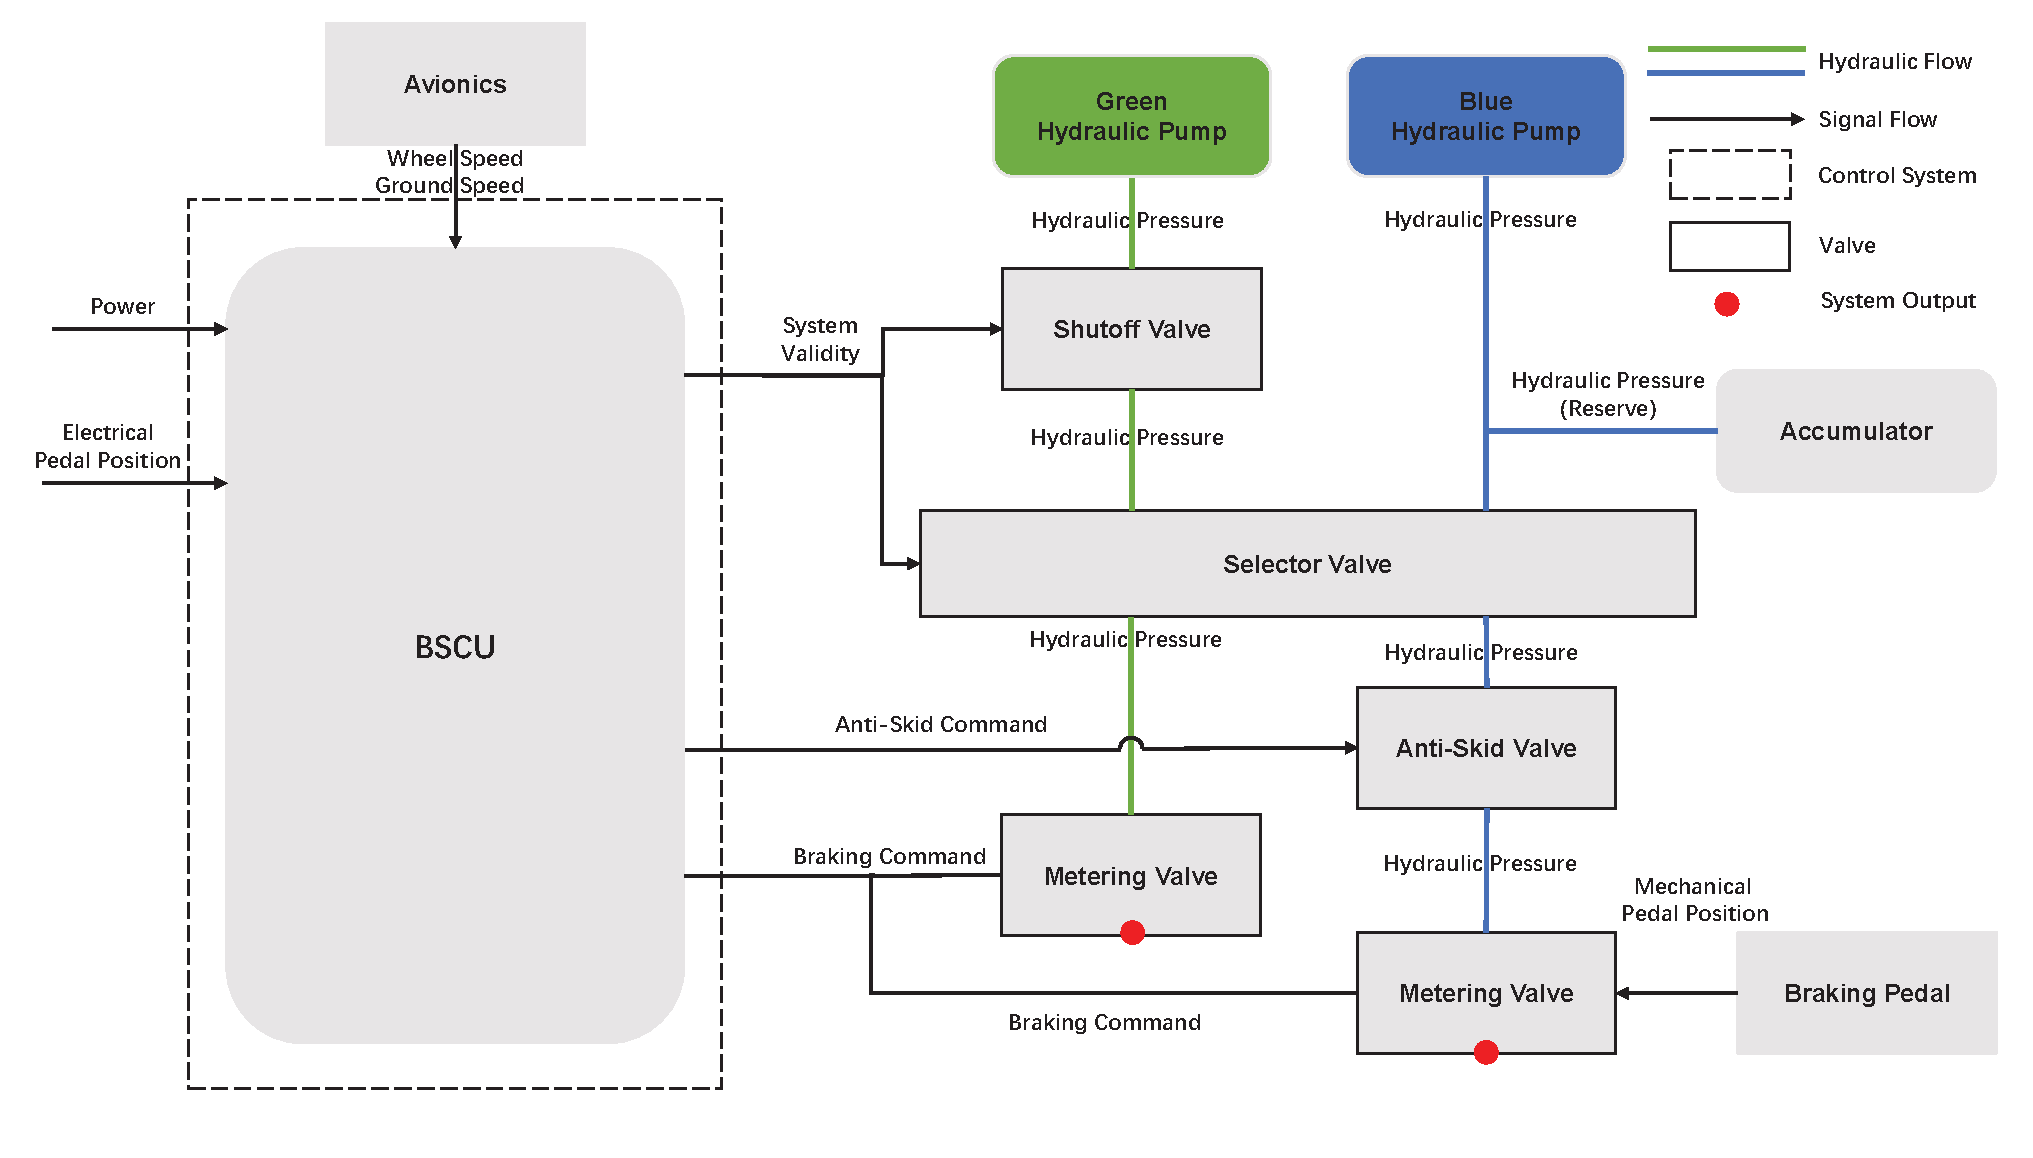
\includegraphics[width=105mm]{figure/Nominal.eps}}
	\caption{The WBS BIP model with the nominal behavior} \label{WBS_BIP_Nominal}
\end{figure}

\subsection{The WBS architecture and nominal behavior}

Fig.~\ref{WBS_BIP_Nominal} shows the WBS BIP model with the nominal behavior. The WBS is composed of an electronic control system and a physical system. The majority of the electronic control system is Braking System Control Unit (BSCU). The WBS receives several signals including the brake pedal position from upper level avionics system and electically forwards them to the BSCU. The BSCU also receives two power inputs from two independent power supply resources. As the result of computation, the BSCU in turn produces the system validity command, anti-skid command and braking command to the physical system. The physical system includes two hydraulic pressure lines which are supplied by the green/blue hydraulic pump respectively.

\emph{Operation Mode.} There are three operation modes for physical system. In \emph{normal mode}, the wheel brake is supported by the main hydraulic circuit, refers to the green hydraulic circuit. In \emph{alternate mode}, the wheel brake is supported by a second hydraulic circuit. This mode is standby and is selected automatically when the normal system fails. An accumulator supplies the \emph{emergency mode} when blue hydraulic supply is lost and the normal mode is not available.

\emph{Braking System Control Unit (BSCU).} According to the AIR6110, for redundancy, the BSCU is composed of two independent channels, each channel has its own power supply and avioncs system inputs. Each channel has a command subsystem and a monitor subsystem. The monitor system generates the system validity command and the command system cauculates the anti-skid command and braking command. The BSCU will make an ultimate judgement call between each command output by the two channels respectively.

\emph{Hydraulic Pump.} In nominal system behavior, both the green and blue hydraulic pumps provide enough hydraulic pressure for their green/blue hydraulic circuit respectively. An accumulator is also a hydraulic pump to provide an emergency reserve of hydraulic pressure for blue hydraulic circuit in emergency mode.

\emph{Shutoff Valve.} The shutoff valve responds the system validity command from BSCU to decide whether to apply the hydraulic pressure to the selector valve in green hydraulic circuit or not. The system validity command is modelled in BIP as a boolean value.

\emph{Selector Valve.} The selector valve control the switch between green and blue hydraulic circuits mechanically. It outputs appropriate pressure from green hydraulic pump, and switches to blue hydraulic circuit as soon as it detects a lack of pressure in the green hydraulic circuit. In BIP model, the component selector valve only outputs pressure from either the green hydraulic circuit input or blue hydraulic circuit input at a time.

\emph{Anti-Skid Valve.} The anti-skid valve follows anti-skid command to control hydraulic pressure to the metering valve. It is used to restrict the hydraulic pressure to the wheel brake in order to prevent locking of the wheel. Wheel skid happens when the wheel is locked but the vehicle keeps a relative slid speed to the ground. We consider a loss of anti-skid function as a fault and will integrate it into nominal BIP model.

\emph{Metering Valve.} Metering valve, or metering servo valve controls pressure to the demanded level and provides regulation for the anti-skid function.

\subsection{The WBS architecture mode in BIP}

According to the AIR6110, the system architecture evolves throughout the development life cycle and is tightly coupled with the requirements development (especially interface requirements) and is not finished until the requirements associated with the architecture have been validated.

We follow the standard to advance our BIP model. As a result, our WBS BIP model has four versions corresponding to the four architectures in the AIR6110. They are numbered from ARCH1 to ARCH4. Each architecture is obtained after design choices of different types.

\emph{ARCH1.} The architecture one is regarded as a high level wheel brake system architecture to be analyzed against the system level functions operational and safety requirements, and any design constraints that have been identified early in the standard.

\emph{ARCH2.} Modified braking system architecture ARCH2 implements the function of ARCH1 and meets various of derived requirements listed in the Wheel Brake System Preliminary Safety Assessment (PSSA). As a feedback of PSSA, things to consider include but are not limited to:

\begin{itemize}
\item The modified architecture shall have at least two independent hydraulic pressure sources.
\item The modified architecture shall have dual channel BSCU and multimode brake operations to provide the required redundancy.
\end{itemize}

\emph{ARCH3.} Following the result of the WBS trade study, the development of architecture three is designed with one BSCU housing two independent systems, each BSCU subsystem has independent command and monitor channels.

%Figure ? shows the iteration from ARCH2 to ARCH3

\emph{ARCH4.} Since architecture three has been simulated and the results of the modelling for each system component are that the schematic of the braking system architecture does not work and there are some mistakes in the schematic. Architecture four is established to avoid the risk of hydraulic supply to wheel brake being possible in normal mode by accumulator. An input is added in ARCH4 to the selector valve corresponding to the validity of the control system. Pedal position signal is input in front of the anti-skid valve in blue hydraulic pressure line and the accumulator is moved to the front of the selector valve.

